\documentclass{beamer}
\usepackage[utf8]{inputenc}

\usetheme{Madrid}
\usecolortheme{default}
\usepackage{amsmath,amssymb,amsfonts,amsthm}
\usepackage{txfonts}
\usepackage{tkz-euclide}
\usepackage{listings}
\usepackage{adjustbox}
\usepackage{array}
\usepackage{tabularx}
\usepackage{gvv}
\usepackage{lmodern}
\usepackage{circuitikz}
\usepackage{tikz}
\usepackage{graphicx}

\setbeamertemplate{page number in head/foot}[totalframenumber]

\usepackage{tcolorbox}
\tcbuselibrary{minted,breakable,xparse,skins}



\definecolor{bg}{gray}{0.95}
\DeclareTCBListing{mintedbox}{O{}m!O{}}{%
	breakable=true,
	listing engine=minted,
	listing only,
	minted language=#2,
	minted style=default,
	minted options={%
		linenos,
		gobble=0,
		breaklines=true,
		breakafter=,,
		fontsize=\small,
		numbersep=8pt,
		#1},
	boxsep=0pt,
	left skip=0pt,
	right skip=0pt,
	left=25pt,
	right=0pt,
	top=3pt,
	bottom=3pt,
	arc=5pt,
	leftrule=0pt,
	rightrule=0pt,
	bottomrule=2pt,
	toprule=2pt,
	colback=bg,
	colframe=orange!70,
	enhanced,
	overlay={%
		\begin{tcbclipinterior}
			\fill[orange!20!white] (frame.south west) rectangle ([xshift=20pt]frame.north west);
	\end{tcbclipinterior}},
	#3,
}
\lstset{
	language=C,
	basicstyle=\ttfamily\small,
	keywordstyle=\color{blue},
	stringstyle=\color{orange},
	commentstyle=\color{green!60!black},
	numbers=left,
	numberstyle=\tiny\color{gray},
	breaklines=true,
	showstringspaces=false,
}
%------------------------------------------------------------
%This block of code defines the information to appear in the
%Title page
\title %optional
{4.11.27}
%\subtitle{A short story}

\author % (optional)
{Hema Havil - EE25BTECH11050}



\begin{document}
	
	\frame{\titlepage}
	\begin{frame}{Question}
		 Find the coordinates of the point where the line through $(4,-3,-4)$ and $(3,-2,2)$ crosses the plane $2x+y+z=6$
         \end{frame}
\begin{frame}{Theoretical Solution}
         Let the given points be P(4,-3,-4) and Q(3,-2,2) then the direction vector along PQ be d, 
         \begin{align}
             \vec{d}=\vec{Q}-\vec{P}=\myvec{3\\-2\\2}-\myvec{4\\-3\\-4}=\myvec{-1\\1\\6}
         \end{align}
         equation of line passing through P,Q be
         \begin{align}
             r(t)=r_0+td
         \end{align}
         where t is a parameter
         \begin{align}
             \vec{r(t)}=\myvec{4\\-3\\-4}+t\myvec{-1\\1\\6}
         \end{align}
         Let the given plane equation be 
         \begin{align}
             \vec{n}^T\vec{x}=c 
         \end{align}
         
         
\end{frame}
\begin{frame}{Theoretical Solution}
         where, 
         \begin{align}
             \vec{n}=\myvec{2\\1\\1}\\
             c=6
         \end{align}
         Consider a point with parameter $t_1$ which is the intersection point then, it satisfies line equation and plane equation 
         \begin{align}
             \vec{r(t_1)}=\myvec{4\\-3\\-4}+t_1\myvec{-1\\1\\6}
         \end{align}
         
         
\end{frame}
\begin{frame}{Theoretical Solution}
Substitute this point in the plane equation 
         \begin{align}
             \vec{n}^T\vec{r_{t_1}}=c
         \end{align}
    \begin{align}
             \myvec{2\;1\;1}\brak{\myvec{4\\-3\\-4}+t_1\myvec{-1\\1\\6}}=6
         \end{align}
         \begin{align}
             1+t_1\brak{5}=6
         \end{align}
         \begin{align}
             5t_1=5
         \end{align}
         \begin{align}
             t_1=1
         \end{align}
         
\end{frame}
\begin{frame}{Theoretical Solution}
    then the intersection point be,
         \begin{align}
             \vec{r_{t_1}}=\myvec{4\\-3\\-4}+\myvec{-1\\1\\6}
         \end{align}
         \begin{align}
             \vec{r_{t_1}}=\myvec{3\\-2\\2}
         \end{align}
\end{frame}
	\begin{frame}[fragile]
	\frametitle{C Code- Computing the unit vector}
	
	\begin{lstlisting}
#include <stdio.h>
void find_intersection(double *result) {
    double P[3] = {4, -3, -4};
    double Q[3] = {3, -2, 2};
    double n[3] = {2, 1, 1};
    double c = 6;
    double d[3];
    for (int i = 0; i < 3; i++) d[i] = Q[i] - P[i];

    double num = c - (n[0]*P[0] + n[1]*P[1] + n[2]*P[2]);
    double den = n[0]*d[0] + n[1]*d[1] + n[2]*d[2];
    double t = num / den;

    for (int i = 0; i < 3; i++)
        result[i] = P[i] + t * d[i];
}

	\end{lstlisting}
\end{frame}

\begin{frame}[fragile]
	\frametitle{Python Code using shared output}
	\begin{lstlisting}
import ctypes
import numpy as np
import matplotlib.pyplot as plt
from mpl_toolkits.mplot3d import Axes3D

# Load the compiled C library
lib = ctypes.CDLL('./4.11.27.so')  # or './intersection.dll' on Windows

# Prepare result array
result = (ctypes.c_double * 3)()
lib.find_intersection(result)

intersection = np.array([result[0], result[1], result[2]])
print("Intersection point:", intersection)


	\end{lstlisting}
\end{frame}
\begin{frame}[fragile]
	\frametitle{Python Code using shared output}
	\begin{lstlisting}	
    # Define line points
P = np.array([4, -3, -4])
Q = np.array([3, -2, 2])
line_points = np.array([P, Q])

# Plane setup
xx, yy = np.meshgrid(np.linspace(0, 5, 10), np.linspace(-5, 5, 10))
zz = 6 - 2*xx - yy  # from plane equation 2x + y + z = 6

# Plot
fig = plt.figure()
ax = fig.add_subplot(111, projection='3d')
\end{lstlisting}
\end{frame}
\begin{frame}[fragile]
  \frametitle{Python Code using shared output}
    \begin{lstlisting}
        ax.plot_surface(xx, yy, zz, alpha=0.5, color='cyan')
ax.plot(line_points[:,0], line_points[:,1], line_points[:,2], color='red', label='Line PQ')
ax.scatter(intersection[0], intersection[1], intersection[2], color='blue', s=50, label='Intersection')

ax.set_xlabel('X')
ax.set_ylabel('Y')
ax.set_zlabel('Z')
ax.set_title('Plot of the Intersection point ')
ax.legend()
plt.show()
    \end{lstlisting}
\end{frame}
\begin{frame}{Plot by python using shared output from c}
	\begin{center}
	\begin{figure}[H]
		\centering
		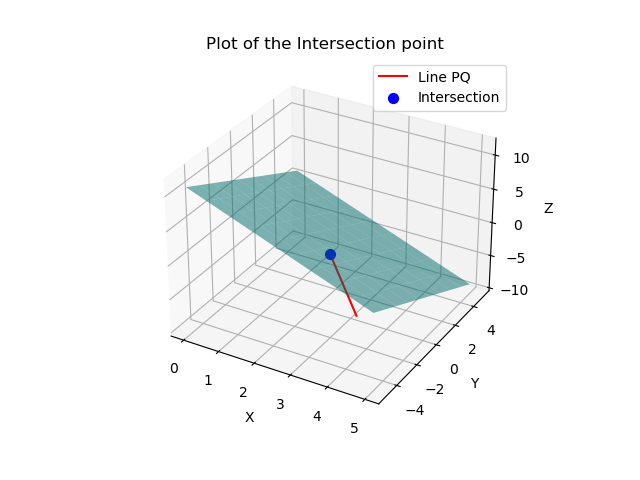
\includegraphics[width = 0.7\columnwidth]{figs/fig1.png}
		\caption{Plot of the Intersection point}
		\label{fig1}
	\end{figure}
	\end{center}
\end{frame}
\begin{frame}[fragile]
     \frametitle{Python code for the plot}
\begin{lstlisting}
    import numpy as np
import matplotlib.pyplot as plt
from mpl_toolkits.mplot3d import Axes3D

# Given data
P = np.array([4, -3, -4])   # Point 1
Q = np.array([3, -2,  2])   # Point 2
# Plane: 2x + y + z = 6
n = np.array([2, 1, 1])     # Normal vector
c = 6
# Direction vector of the line
d = Q - P
# Parameter t for intersection point
t = (c - np.dot(n, P)) / np.dot(n, d)
# Intersection point
R = P + t * d
print("Intersection point:", R)
\end{lstlisting}
\end{frame}
\begin{frame}[fragile]
   \frametitle{Python code for the plot}
    \begin{lstlisting}
# --- Plotting the line, plane, and intersection point ---
fig = plt.figure()
ax = fig.add_subplot(111, projection='3d')

# Generate the plane surface
xx, yy = np.meshgrid(np.linspace(0, 5, 10), np.linspace(-5, 5, 10))
zz = 6 - 2*xx - yy  # from plane equation 2x + y + z = 6

# Plot the plane
ax.plot_surface(xx, yy, zz, alpha=0.5, color='cyan')

# Plot the line passing through P and Q
line_points = np.array([P, Q])
ax.plot(line_points[:,0], line_points[:,1], line_points[:,2],
        color='red', label='Line PQ')
 \end{lstlisting}
\end{frame}
\begin{frame}[fragile]
  \frametitle{Python code for the plot}
    \begin{lstlisting}
# Plot the intersection point
ax.scatter(R[0], R[1], R[2], color='blue', s=50, label='Intersection Point')

# Annotate points
ax.text(P[0], P[1], P[2], 'P(4,-3,-4)', color='black')
ax.text(Q[0], Q[1], Q[2], 'Q(3,-2,2)', color='black')
ax.text(R[0], R[1], R[2], f'R({R[0]:.1f},{R[1]:.1f},{R[2]:.1f})', color='blue')

# Labels
ax.set_xlabel('X-axis')
ax.set_ylabel('Y-axis')
ax.set_zlabel('Z-axis')
ax.set_title('Intersection of Line and Plane')

ax.legend()
plt.show()
    \end{lstlisting}
\end{frame}
 \begin{figure}
     \centering
     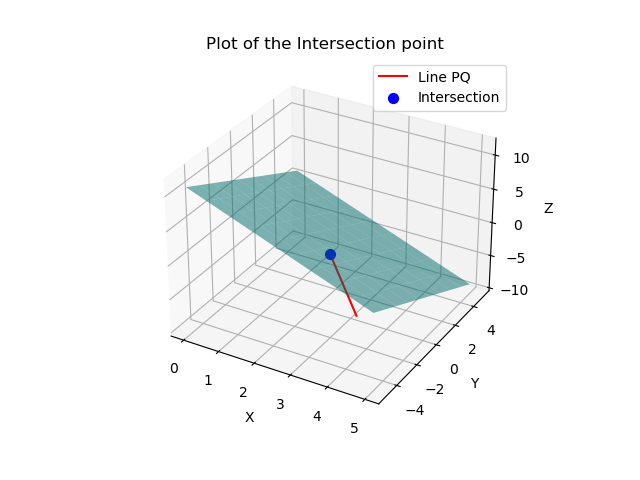
\includegraphics[width=0.7\linewidth]{figs/fig1.png}
     \caption{Plot of the Intersection point }
     \label{fig1}
 \end{figure}
\end{document}
